\documentclass{article}
\usepackage[utf8]{inputenc}

%additional usepackages
\usepackage{amsmath}
\usepackage{eufrak}
\usepackage{tikz}
\usepackage{ amssymb }
\usepackage{import}
\usepackage[ruled,vlined]{algorithm2e}
\usepackage{booktabs}
\usepackage[capposition=top]{floatrow}
\usepackage{scrextend}
\usepackage{csquotes}
\usepackage{graphicx}
\usepackage{pdfpages}

% bibliography
\usepackage[backend=biber, citestyle=authoryear]{biblatex}
\addbibresource{acfs.bib}


% margins
\usepackage[margin=1.05in]{geometry}

%new commands
\newcommand{\ances}{AN_{A}^{\mathcal{G}}}
\newcommand{\anc}{\mathbf{AN}^{\mathcal{G}}}
\newcommand{\dec}{\mathbf{DE}^{\mathcal{G}}}
\newcommand{\dsep}{\text{ \textit{d}-sep }}
\newcommand{\dseperation}{\text{ \textit{d}-seperation}}
\newcommand{\nodes}{\mathbf{V}}
\newcommand{\parents}{\mathbf{PA}^{\mathcal{G}}}
\newcommand{\parentsNew}{\mathbf{PA}^{\mathcal{G^{*}}}}
\newcommand{\summ}{\frac{1}{n}\sum_{i=1}^{n}}


\newcommand{\children}{\mathbf{CH}^{\mathcal{G}}}

\newcommand{\graph}{\mathfrak{C}}
\newcommand{\E}{\mathbb{E}}
\newcommand{\std}{\mathbf{std}}
\newcommand{\R}{\mathbb{R}}
\newcommand{\G}{\mathcal{G}}
\newcommand{\lra}{\Leftrightarrow}

\newcommand{\la}{\leftarrow}
\newcommand{\ra}{\rightarrow}

\newcommand{\rp}{\right)}
\newcommand{\lp}{\left(}

%%%% INDEPDENT SIGN %%%%

\makeatletter
% Taken from http://ctan.org/pkg/centernot
\newcommand*{\centernot}{%
  \mathpalette\@centernot
}
\def\@centernot#1#2{%
  \mathrel{%
    \rlap{%
      \settowidth\dimen@{$\m@th#1{#2}$}%
      \kern.5\dimen@
      \settowidth\dimen@{$\m@th#1=$}%
      \kern-.5\dimen@
      $\m@th#1\not$%
    }%
    {#2}%
  }%
}
\makeatother

\newcommand{\independent}{\perp\mkern-9.5mu\perp}
\newcommand{\notindependent}{\centernot{\independent}}

%%%%% INDEPENDENT SIGN END %%%%%

\newcommand{\X}{\mathbf{X}}
\newcommand{\Ls}{\mathbf{L}}
\newcommand{\D}{\mathbf{D}}
\newcommand{\W}{\mathbf{W}}

\newcommand{\x}{\mathbf{x}}
\newcommand{\ls}{\mathbf{l}}
\newcommand{\ds}{\mathbf{d}}
\newcommand{\w}{\mathbf{w}}

\newcommand{\rr}{\mathbf{r}}
\newcommand{\RR}{\mathbf{R}}

\newcommand{\ones}{\mathbf{1}}

\DeclareMathOperator*{\argmax}{arg\,max}
\DeclareMathOperator*{\argmin}{arg\,min}


\setlength{\parindent}{0em}
\setlength{\parskip}{0.25cm}

\title{Stock Picking In An Environment Of Structural Breaks}
\author{Jeppe Søndergaard Johansen (pcv439)}
\date{August 2019}

\makeindex

\begin{document}


\includepdf[pages={1}]{frontpage/frontpage.pdf}

\maketitle


\begin{abstract}
This paper investigates reinforcement learning as a solution method for dynamic models. A discrete time, finite horizon, discrete choice model of female labour supply and fertility is formulated, and the model is solved using value function iteration and two reinforcement learning methods, namely deep Q-learning and double deep Q-learning. After estimating the model using method of simulated moments, and finding the simple model inadequate to describe data from Statistic Denmark, the model is extended. The extension consists of 14 + 1 states. The extended model is solved only using double deep Q-learning and estimated using simulated method of moments. The results of the extended model convincingly matches data from Statistics Denmark and contemporary findings by \textcite{kleven_children_2019}. I conclude that the field of economics should further investigate reinforcement learning, as it allows solving dynamic models with high dimensional state space.
\end{abstract}


\pagebreak

\tableofcontents

\pagebreak

\section{Introduction} 

The last 10 years have lead to numerous breakthroughs within the field of machine learning, among them especially the subfield of reinforcement learning has experienced great leaps. In 2013 the company DeepMind achieved super human performance in various Atari games \parencite{mnih_playing_2013}. In 2018 the same company beat professional human players in the board game Go, a feat which was not deemed possible in a foreseeable future \parencite{silver_general_2018}, and as late as 2019 DeepMind showed that an reinforcement learning agent was able to play the game of Star Craft 2 on the same level as the best human players \parencite{vinyals_grandmaster_2019}. All the games mentioned can be considered dynamical models. Dynamic models play a central role within the field of economics. The results imply a new way of solving dynamic economic models using reinforcement learning.

Dynamical models usually involve agents that take sequential actions, trying to maximize the cumulative utility from these actions. This class of economic models conform to a set of properties economists like: They have a micro foundation - agents are utility maximizing. They model time, allowing for agents to foresee the future, and act in accordance to their expectations. Some dynamic models can be solved  analytically. This is true for the canonical Ramsey model. However when the scope of the dynamic model grows, different approaches is necessary. Dynamic programming is usually the tool utilized for solving such models.  Even though dynamic programming is a flexible tool it do have its limitations. Solving a model using dynamic programming, requires a limited sized state space, otherwise the computation involved becomes infeasible. In practice this leaves high dimensional dynamic models impossible to solve using contemporary techniques. Deep reinforcement learning allows for solving such models. Because these techniques are relatively novel, they have not yet been introduced into the field of economics. Deep reinforcement learning, does unfortunately not guarantee that the solution converges to the global maximum, but results have shown that learning is possible in hard, high dimensional environments.

This paper uses the aforementioned techniques to investigate the effect of children on female labour supply. Inspired by the model specification of \textcite{francesconi_joint_2002} and \textcite{adda_career_2011} I formulate an discrete time, finite horizon model that models discreet female labour supply and its relationship to fertility. First a simple model is formulated, where women can choose the number of supplied hours, letting fertility be exogenous, with an income process following the Mincer equation of human capital. The husband of the household, is assumed to follow a deterministic path both with regards to number of hours supplied to the labour force, and with the wage rates they receive. Households are assumed to face a budget constraint, that neither allow for borrowing or saving. Utility is assumed to be a function of leisure and consumption, and children are assumed to reduce leisure by mirroring additional work for the woman, that is not financially compensated. Later an extension to the original model is presented with exogenous education combined with a transfer system for women in the education system. Additionally the extension tracks children on an individual level.

Using three different solution methods: value function iteration, deep Q-learning and double deep Q-learning I solve the simple model. I show that one can get comparable performance using deep reinforcement learning compared to using value function iteration solution methods, yielding a new way to solve more complex dynamic models. The parameters of the Mincer equation are calibrated using data from Statistics Denmark . The model is estimated using method of simulated moments, where a simple grid search approach is applied due to fact the optimization problem being one dimensional. The extended model is only solved using double deep Q-learning. Again the model is estimated using method of simulated moments and grid search. The data used for the optimization is from Statistics Denmark.

My two main findings are: 1) Deep reinforcement learning can yield comparable performance to value function iteration solution methods. Considering this allows for solving dynamic models with high dimensional state space, I argue these methods should be explored further in the field of economics. 2) Simulating from the estimated model, I find the initial simple model is not able fit the data, whereas the extended model does fit the data surprisingly well. Both participation rates and average number of supplied hours to labour force, are surprisingly close to what the data from Statistics Denmark suggest. Comparing to  \textcite{kleven_children_2019}, this paper finds results very similar with regards to earnings, participation rate, supplied hours to the labour force and wage rates, when women gives birth to a child.

The paper follows the structure: A literature review is conducted highlighting the main findings and articles of endogenous female labour supply and the effect of children. A model is formulated based on key takeaways from the literature. The parameters of the income process is calibrated using data from Statistics Denmark. Next, I introduce the reader to both reinforcement learning and deep learning. Settling on three different solution methods i solve and estimate the model. I go on to extend the model, and solve it using double deep Q-Learning. I end by comparing the results to contemporary findings, and data from Statistics Denmark.

\section{Data}

\input{chapters/model.tex}

\input{chapters/simulation.tex}

\input{chapters/algorithms.tex}

\input{chapters/analysis.tex}

\input{chapters/discusion.tex}

\section{Conclusion}

This paper has tried to establish how reinforcement learning can be used to solve dynamic models. I show that using these solution methods allow for solving models otherwise computationally infeasible. I argue that when using such methods, there is no guarantee of finding the optimal policy, and there exists a real risk of ending up in local maxima. Furthermore have I presented an economic model of exogenous fertility and endogenous female labour supply, that can give a surprisingly good fit to data, and show comparable long term penalties for female participation rates, earnings, wage rates and hours worked to contemporary findings by \textcite{kleven_children_2019}, when a household gets a child. 

The first part of the paper, I draw on the literature of female labour supply and fertility to formulate a simple dynamic model of female labour supply and fertility, tracking households over the life cycle, where women can supply a discreet number of hours to the labour force. I use aggregate data for Statistics Denmark to calibrate the parameters of the income process. For this task I assume that the households follows a deterministic strategy with regards to labour supply. I find, the model seem to approximate the income paths of both men and women very well. Next, I present the reader for reinforcement learning and deep learning allowing the reader to have an understanding of the algorithms used for solving the models presented in this paper.  I go on to present three different solution methods: Value function Iteration using deep neural networks for value function approximation, Deep Q-learning and Double Deep Q-Learning. I find that these three solution methods have comparable performance, but the model does not seem to fit the data well! Next i formulate an extension of the inadequate model, and use Double Deep Q-learning as solution method. I estimate the extra parameters using method of simulated moments. Simulating from the model using the estimated parameters, I find that both the participation rate and the average number of supplied hours to the labour force is comparable to what is found in data. Next i compare event graphs to those found by \textcite{kleven_children_2019} and find striking similarities, finding that women do experience a real penalty when getting a child.



\newpage
\printbibliography

\newpage
\section*{Appendix}

\listoffigures
\listoftables

\begin{figure}
    \centering
    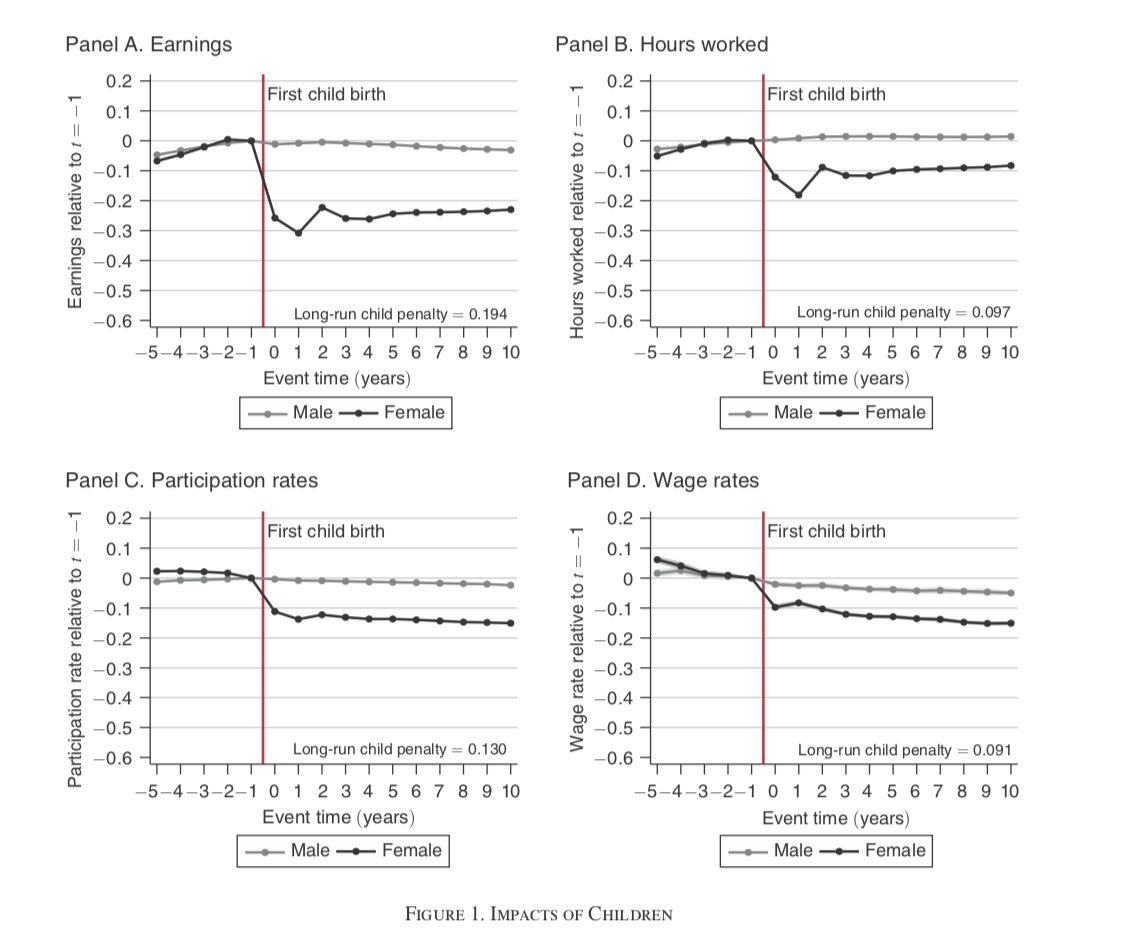
\includegraphics[scale=0.3]{figures/kleven_10_years_impact.png}
    \caption{Event Graphs of \textcite{kleven_children_2019}}
    \label{fig:my_label}
\end{figure}


\end{document}
